\graphicspath{{./figures}}

\section{Tracking and Pointing}

\subsection{Open-Loop}

In order to test the GPS pointing and open-loop tracking, a map was printed with lines pointing to nearby locations from a pre-determined location. The ground station was then placed on top of this map at this location and calibrated (as described in Appendix \ref{sec:appendix_mount_calibration}). This test had multiple goals i.e. to test the mount transfer function, the GPS co-ordinate pointing, and the flight path tracking. An image of the test setup is shown in Figure \ref{fig:pointingTestSetup}.

Flight path data containing the map locations was then uploaded, and the azimuthal angle was qualitatively confirmed to point in the map directions using a ruler. The elevation angle was measured using a protractor and found to be within $5^\circ$ of the expected angle. The system was also found to successfully point towards the commanded locations at the desired times. Since the beamwidth of the antenna is on the order of $60^\circ$, it was decided not to use a more accurate testing technique, since it is clear the system was functional at least within requirements.

\subsection{Closed-Loop}\label{sec:closed_loop_testing}
\begin{figure}[!tb]
  \begin{minipage}{.49\textwidth}
    \centering
    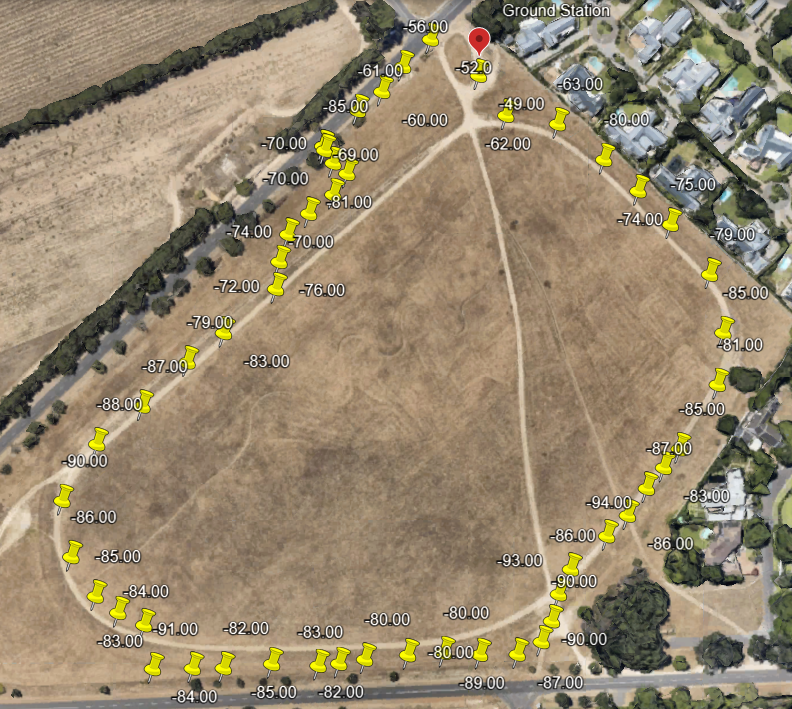
\includegraphics[width=0.95\linewidth]{gpsTrackingMap}
    \caption{GPS Tracking Locations and RSSI Values}
    \label{fig:gpsTrackingMap}
  \end{minipage}
  \begin{minipage}{.49\textwidth}
    \centering
    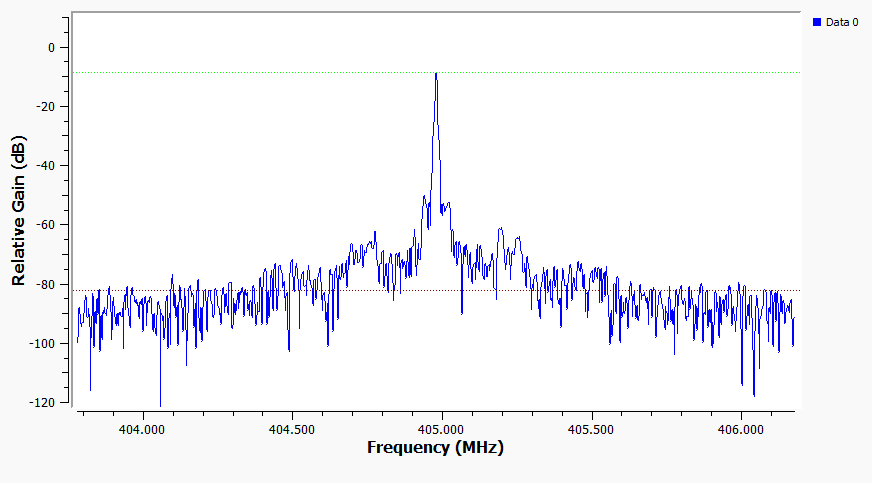
\includegraphics[width=1.0\linewidth]{radiosondeSpectrum}
    \caption{Received Radiosonde Signal Spectrum}
    \label{fig:radiosondeSpectrum}
  \end{minipage}
\end{figure}

Closed-loop GPS tracking was tested on an open field at \SI{300}{m} range. The PQ unit was carried around the field at a walking speed of $\SI{2}{m.s^{-1}}$ while transmitting its GPS location. Both the RSSI, and the antenna pointing direction, were recorded. The system was observed to successfully track the transmitter around the field without noticeable delay. The $90^\circ$ turn created by the furthest ends of the field creates an approximate 500 m path, which was covered in 100 s. This results in a turning rate of around $0.9 ^ \circ$, which meets the requirement of $0.015 ^ \circ$. The tracking was observed to be successful until the target reached a distance of around 10 m, where the pointing direction became unpredictable. This is attributed to the low accuracy of the GPS modules.